\icode{N24S-MD-SI-L2-261113-001}
\nceeID[4]{2024江苏}{4}
倾角为\(\theta\)的传送带以恒定速率\(v_0\)顺时针转动。\(t = 0\)时在传送带底端无初速轻放一小物块，如图所示。\(t_0\)时刻物块运动到传送带中间某位置，速度达到\(v_0\)。不计空气阻力，则物块从传送带底端运动到顶端的过程中，加速度\(a\)、速度\(v\)随时间\(t\)变化的关系图线可能正确的是\paren[]
	
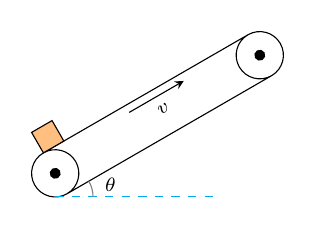
\begin{tikzpicture}[>=stealth,font=\scriptsize]
	\begin{scope}[rotate=30]
		\draw (0,0) circle(.3) (3,0) circle(.3) (0,.3)--(3,.3) (0,-.3)--(3,-.3);
		\fill (0,0) circle(.07) (3,0) circle(.07);
		\draw[fill=orange!50] (0,.3) rectangle(.3,.6);
		\draw[->] (1.2,.2)--node[below,rotate=30]{\(v\)}(2,.2);
	\end{scope}
	\draw[dashed,cyan] (0,-.3)--(2,-.3);
	\draw[gray] ({.3*tan(15)+.4},-.3) arc(0:30:.4);
	\node at(.7,-.15){\(\theta\)};
\end{tikzpicture}

\begin{tikzpicture}[>=stealth,font=\scriptsize]
	\begin{scope}
		\draw[->,blue] (0,0)--(3,0)node[below]{\(t\)};
		\draw[->,blue] (0,0)--(0,2.5)node[right]{\(a\)};
		\node[blue] at(-.2,-.2){\(O\)};
		\draw[magenta] (0,1.4)--(2.6,1.4);
		\draw[dashed,cyan] (1.3,1.3)--(1.3,0)node[below,blue]{\(t_0\)};
		\node at(1.5,-.8){\normalsize\(A\)};
	\end{scope}
	\begin{scope}[xshift=3.7cm]
		\draw[->,blue] (0,0)--(3,0)node[below]{\(t\)};
		\draw[->,blue] (0,0)--(0,2.5)node[right]{\(a\)};
		\node[blue] at(-.2,-.2){\(O\)};
		\draw[magenta] (0,1.4)--(1.3,1.4)--(2.6,0);
		\draw[dashed,cyan] (1.3,1.3)--(1.3,0)node[below,blue]{\(t_0\)};
		\node at(1.5,-.8){\normalsize\(B\)};
	\end{scope}
	\begin{scope}[xshift=7.4cm]
		\draw[->,blue] (0,0)--(3,0)node[below]{\(t\)};
		\draw[->,blue] (0,0)--(0,2.5)node[right]{\(v\)};
		\node[blue] at(-.2,-.2){\(O\)};
		\draw[magenta] (0,0)--(1.3,1.4)--(2.6,1.4);
		\draw[dashed,cyan] (1.3,1.3)--(1.3,0)node[below,blue]{\(t_0\)} (0,1.4)node[left,blue]{\(v_0\)}--(1.3,1.4);
		\node at(1.5,-.8){\normalsize\(C\)};
	\end{scope}
	\begin{scope}[xshift=11.1cm]
		\draw[->,blue] (0,0)--(3,0)node[below]{\(t\)};
		\draw[->,blue] (0,0)--(0,2.5)node[right]{\(v\)};
		\node[blue] at(-.2,-.2){\(O\)};
		\draw[magenta] (1.3,1.4)--(2.6,1.4);
		\draw[domain=0:1.3,magenta] plot(\x,{1.5-1.5*exp(-2.08*\x)});
		\draw[dashed,cyan] (1.3,1.3)--(1.3,0)node[below,blue]{\(t_0\)} (0,1.4)node[left,blue]{\(v_0\)}--(1.3,1.4);
		\node at(1.5,-.8){\normalsize\(D\)};
	\end{scope}
\end{tikzpicture}
\begin{answer}
    C\qquad 提示：
\end{answer}